\section{General Framework Contributions}


\section{Reach with No Obstacles}

\section{Grasping}
  \begin{figure}[H] 
    \centering
    \includegraphics[scale=0.6]{assets/cam-comb/grasp-simple/Z-tuning-normal-old-policy.png}
    \caption{Final Distance for Current Policy (less linear layers in MLP gripper head)}
  \end{figure}

  \begin{figure}[H] 
    \centering
    \includegraphics[scale=0.6]{assets/cam-comb/grasp-simple/Z-tuning-normal-old-policy-success.png}
    \caption{Success Count for Current Policy (less linear layers in MLP gripper head)}
  \end{figure}

  \begin{figure}[H] 
    \centering
    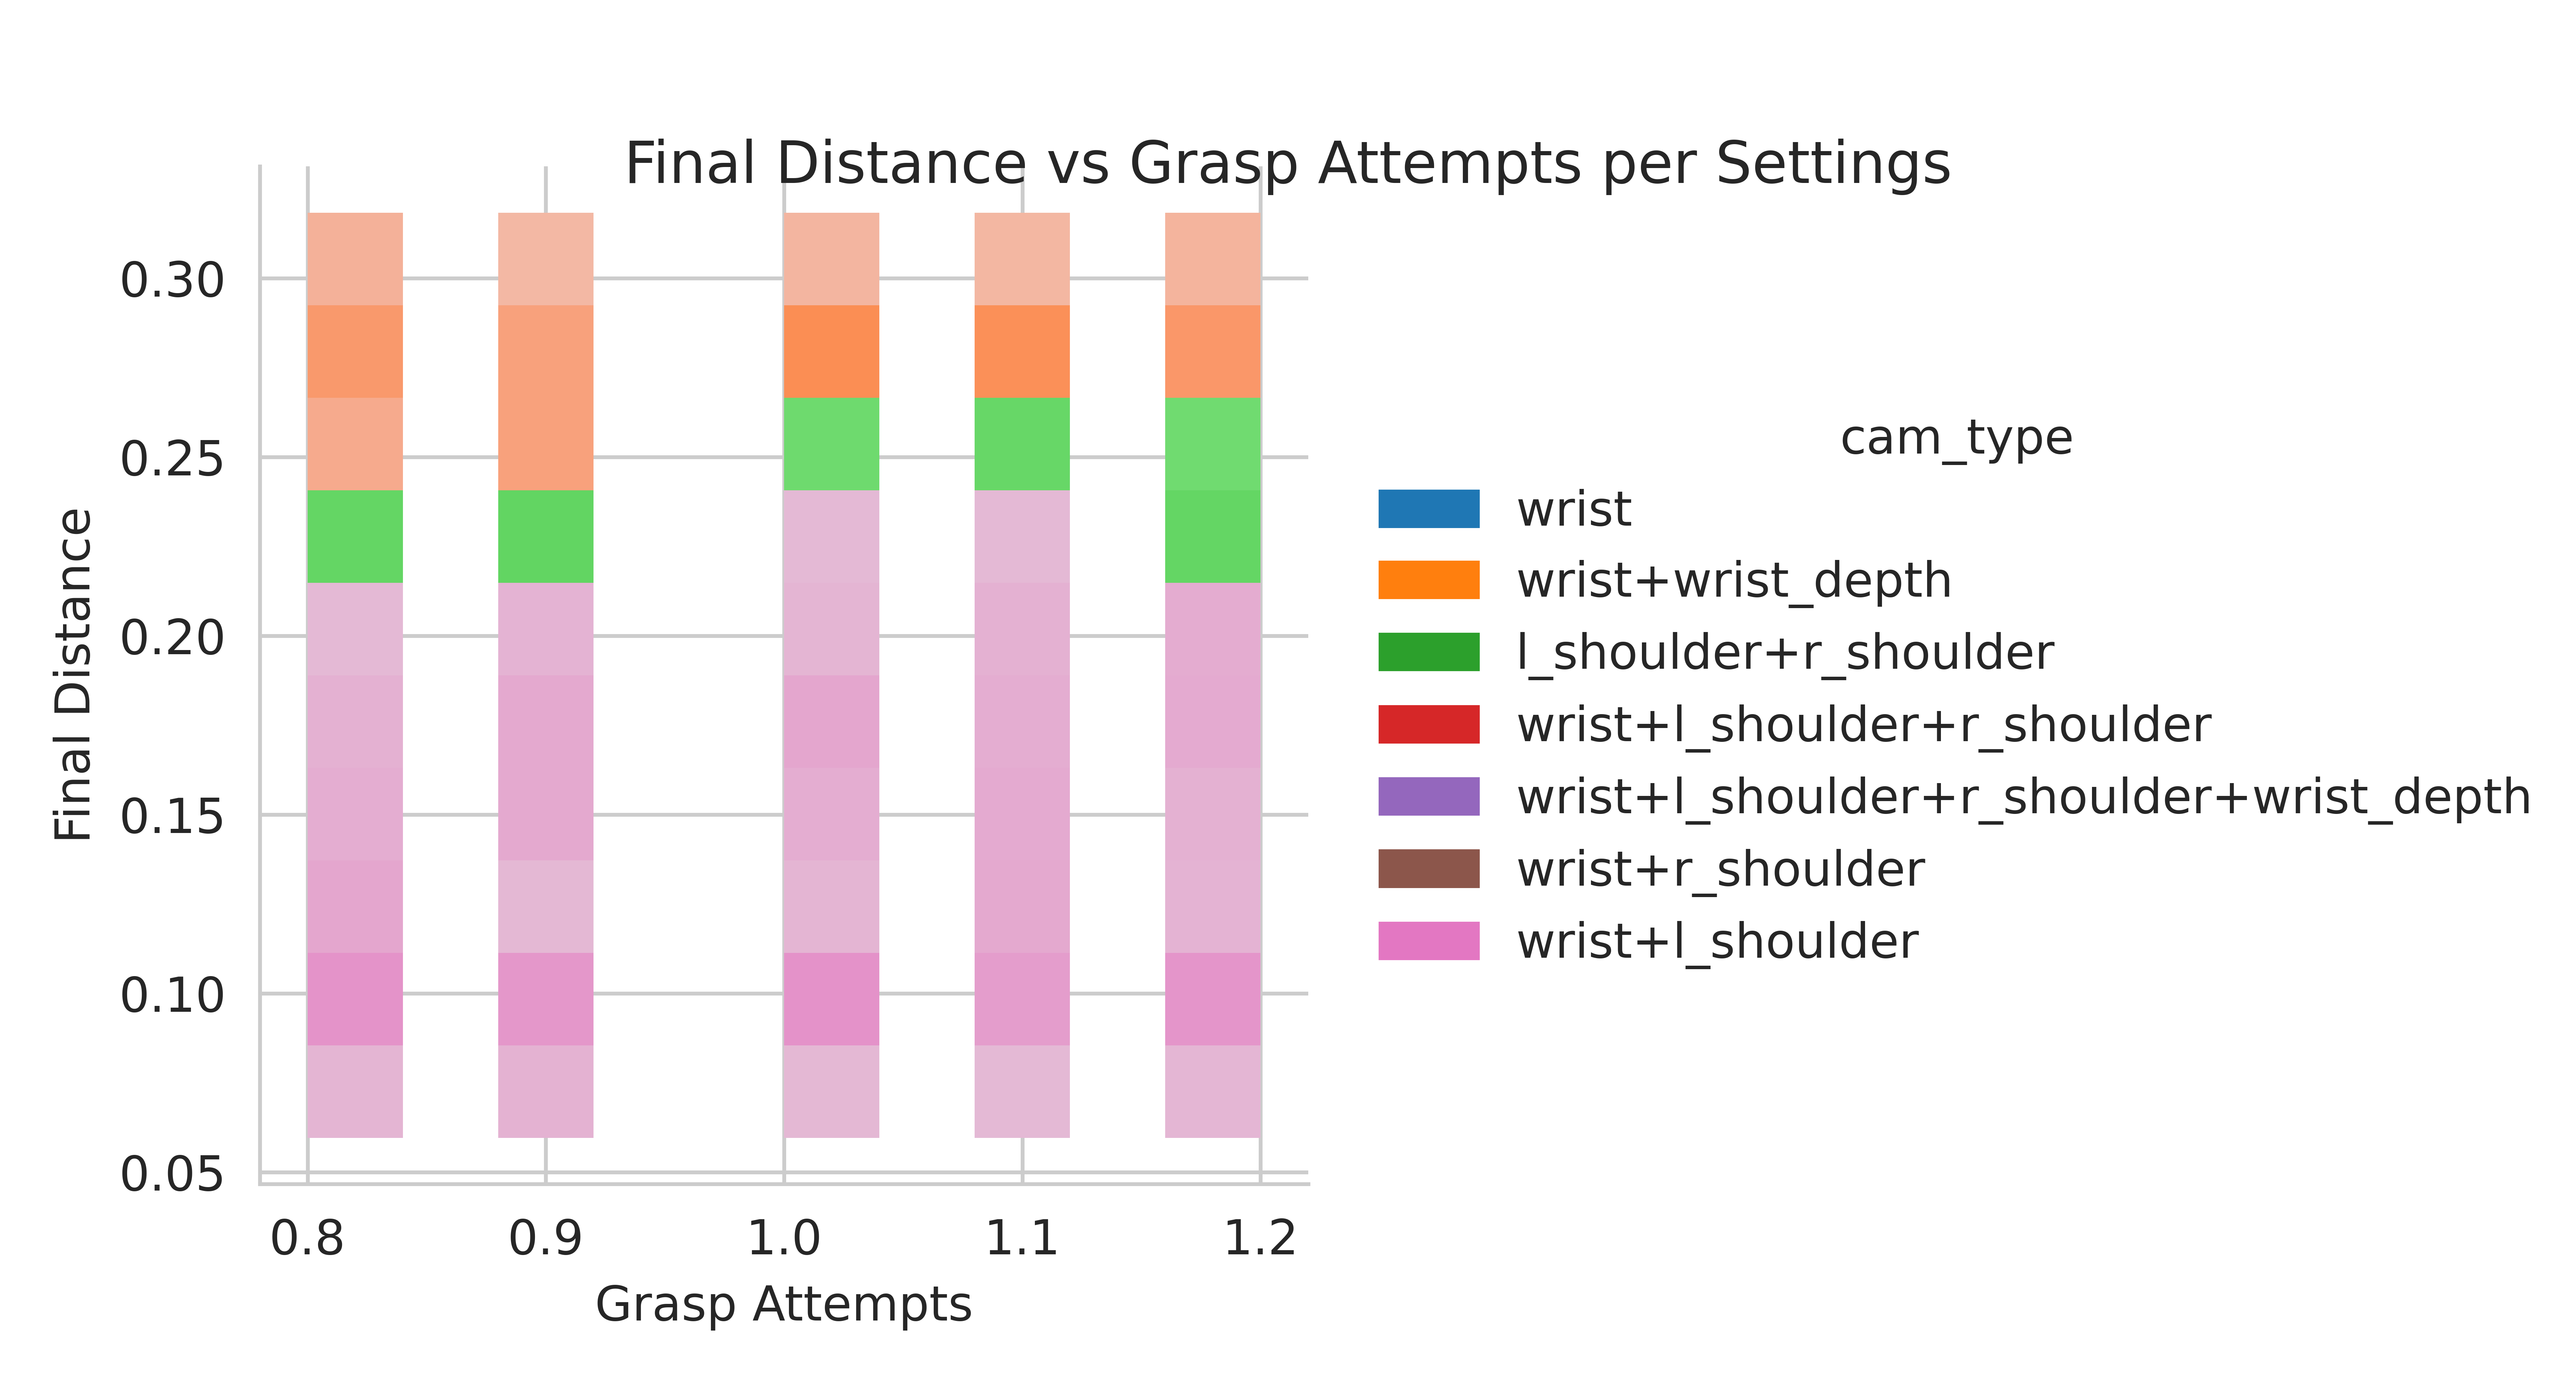
\includegraphics[scale=0.6]{assets/cam-comb/grasp-simple/Z-tuning-normal-old-policy-lambda-dist-hist-hue-cams.png}
    \caption{}
  \end{figure}


  \begin{figure}[H] 
    \centering
    \includegraphics[scale=0.5]{assets/cam-comb/grasp-simple/Z-tuning-normal-old-policy-lambda-dist-hist.png}
    \caption{}
  \end{figure}

  \begin{figure}[H] 
    \centering
    \includegraphics[scale=0.6]{assets/cam-comb/grasp-simple/Z-tuning-normal-old-policy-retry-success.png}
    \caption{}
  \end{figure}

  \begin{figure}[H]
    \centering
    \includegraphics[scale=0.6]{assets/cam-comb/grasp-simple/Z-tuning-normal-old-policy-retry-dist-hist.png}
    \caption{hist}
  \end{figure}

  \begin{figure}[H]
    \centering
    \includegraphics[scale=0.6]{assets/cam-comb/grasp-simple/Z-tuning-normal-old-policy-retry-dist-kde.png}
    \caption{KDE}
  \end{figure}\todo{maybe remmove, not sure what this really is saying}

  \begin{figure}[htpb]
    \centering
    \includegraphics[scale=0.6]{assets/cam-comb/grasp-simple/Z-last-k-dist.png}
    \caption{K Mask Final Distances}
  \end{figure}

  \begin{figure}[htpb]
    \centering
    \includegraphics[scale=0.6]{assets/cam-comb/grasp-simple/Z-last-k-mindist.png}
    \caption{K Mask Minimum Distances}
  \end{figure}

  \begin{figure}[htpb]
    \centering
    \includegraphics[scale=0.6]{assets/cam-comb/grasp-simple/Z-last-k-success.png}
    \caption{K Mask Success}
  \end{figure}

\section{Reach with Obstacles}
  \begin{figure}[H]
    \centering
    \includegraphics[scale=0.6]{assets/cam-comb/reach-obs/Z-ro_random-Final-dist.png}
    \caption{Final Distances}
  \end{figure}

  \begin{figure}[H]
    \centering
    \includegraphics[scale=0.6]{assets/cam-comb/reach-obs/Z-ro_random-Minimum-dist.png}
    \caption{Minimum Distances}
  \end{figure}

  \begin{figure}[H]
    \centering
    \includegraphics[scale=0.6]{assets/cam-comb/reach-obs/Z-ro_random-success.png}
    \caption{Success Rate}
  \end{figure}

  \begin{figure}[htpb]
    \centering
    \includegraphics[scale=0.6]{assets/cam-comb/reach-obs/Z-ro_random-obs-dist.png}
    \caption{Reach `Random' and `IndRandom' Final Distannce}
  \end{figure}

  \begin{figure}[htpb]
    \centering
    \includegraphics[scale=0.6]{assets/cam-comb/reach-obs/Z-ro_random-obs-mindist.png}
    \caption{Reach `Random' and `IndRandom'}
  \end{figure}

  \begin{figure}[htpb]
    \centering
    \includegraphics[scale=0.6]{assets/cam-comb/reach-obs/Z-ro_random-obs-trials-success.png}
    \caption{Running \emph{obs dataset} with different batch sizes}\label{apx:Z-ro_random-obs-trials-success}
  \end{figure}